\section{Bestimmung und Validierung von Materialparametern}
\label{Kapitel:Parameter}
Um eine realistische Simulation zu ermöglichen, ist es notwendig die verwendeten Modelle möglichst genau an Messdaten der realen Mörtel anzupassen. Dazu können die materialabhängigen Parameter in den Modellen variiert werden.\\
Für einige der Mörtel wurden die Parameter, die im verwendeten Modell~\eqref{eq:modHB} vorkommen, schon in früheren Arbeiten bestimmt. \\
Einerseits wurden aber in der Zwischenzeit neue Mörtel entwickelt und andererseits ist es wünschenswert, ein Tool zur automatischen Bestimmung dieser Parameter zu haben das unabhängig von Drittanbietern in Form von Lizenzen und Support ist. \\
Dies wurde mithilfe einer Kombination aus \openfoam{} und der Programmiersprache Python umgesetzt.
%
\subsection{Rheometer}
Rheometer sind Geräte, mit denen man die Fliesskurve von nicht-Newtonschen Fluiden experimentell bestimmen kann.
Dabei wird das Fluid in eine stationäre, laminare Schichtenströmung versetzt, die es erlaubt anhand einer vom Gerät abhängigen Messgrösse die Viskosität abhängig von der Scherrate zu bestimmen.
Die Messungen wurden von einem Hilti-internen Rheologen durchgeführt. Verwendet wurden zwei Messgeräte, ein Platte-Platte Rheometer und ein Kapillarrheometer.
%
\subsubsection{Platte-Platte Rheometer}
\label{Kapitel:Parameter:PlattePlatteRheo}
Das Platte-Platte Rheometer besteht aus zwei zylindrischen Platten, die so montiert sind dass zwischen ihnen ein schmaler, ebenfalls zylinderförmiger Spalt entsteht. \todo{Bild Rheometer}
Die Flüssigkeit wird in diesem Scherspalt platziert, der in radialer Richtung von einem Ring abgeschlossen werden kann. Beim Messvorgang wird die eine Platte fixiert, die andere mit einer vorgegebenen Geschwindigkeit $\Omega$ gedreht.
Dabei wird das benötigte Drehmoment gemessen, das für die Drehgeschwindigkeit aufgewendet werden muss.

Die verwendete Formel dazu lautet:
\begin{equation}
    \label{eq:platterheovisko}
    \eta\left( \gammap \right) = \frac{2M}{\pi R^3 \gammap}\left( \frac{3+n}{4} \right) \text{ mit } n=\frac{d\ln M}{d\ln\gammap}
\end{equation}
Wobei $M$ das notwendige Drehmoment ist und $R$ der Radius der verwendeten Platten.
Für eine Herleitung dieser Formel wird auf \cite{introtorheo} verwiesen.

Das Platte-Platte Rheometer eignet sich ebenfalls dazu, zeitabhängige Effekte wie die Relaxationszeit eines viskoelastischen Fluids zu messen.
Dazu wird die obere Platte nicht mit einer konstanten Geschwindigkeit bewegt, sondern mit einer schwingungsähnlichen Drehung auf die eine oder die andere Seite bewegt.\\
Bei diesem Vorgang, der Oszillationsmessung genannt wird, kann anhand der resultierenden, nicht stationäre Strömung über die Messung des Widerstandes eine Abschätzung der der Schwinungsmodi der Flüssigkeit gemacht werden.

Die sinusförmige Deformation $\gamma$ des Fluides verursacht dabei einen ebenfalls sinusförmigen Widerstand, der durch eine Schubspannung $\tau$ im Fluid zustandekommt.\\
Bei einem ideal viskosem Fluid ist dieser mit der Deformation um 90$^\circ$ Phasenverschoben, da der Widerstand proportional zur Schergeschwindigkeit $\gammap$ der Flüssigkeit ist.\\
Bei einem ideal elastischem Material ist der Widerstand in Phase mit der Deformation, da er direkt proportional zur Verzerrung $\gamma$ des Materials ist.\\
Ein viskoelastisches Fluid besitzt die Eigenschaften beider Materialien und hat deshalb einen Antworts-Widerstand, der um einen Winkel zwischen 0 und 90$^\circ$ phasenverschoben ist. Dieser Zusammenhang ist in Abbildung~\ref{fig:schwingungsmodi} dargestellt.

Diese Beziehungen können als Zusammenhang zwischen Schubspannung $\tau$ und Zeit $t$ ausgedrückt werden:
\begin{align}
    \label{eq:schwingungsmodi}
    \tau\left( t \right)&=G'\cdot\hat{\gamma}\cdot \sin\left( \omega\cdot t \right) && \text{elastisch}\\
    \tau\left( t \right)&=\eta\cdot\omega\cdot\hat{\gamma}\cdot \cos\left( \omega\cdot t \right)&& \text{viskos}\\
    \tau\left( t \right)&=G'\cdot\hat{\gamma}\cdot \sin\left( \omega\cdot t \right)+G''\cdot\hat{\gamma}\cdot \cos\left( \omega\cdot t \right)&& \text{viskoelastisch}
\end{align}
Dabei ist $\omega$ die Kreisfrequenz und $\hat\gamma$ die Amplitude der am Rheometer angelegten Schwingung, $\eta$ die Viskosität des Fluids und $G'$ das Elastizitätsmodul des elastischen Materials. Der Term $\eta\cdot\omega$ wird auch als Verlustmodul $G''$ bezeichnet.

Anhand von $G'$ und $G''$ können die viskoelastischen Eigenschaften wie z.B. die Relaxationszeit eines Fluids bestimmt werden.

\begin{figure}
    \centering
    \subfloat[Auslenkung $\gamma$ und Schergeschwindigkeit $\gammap$]{
    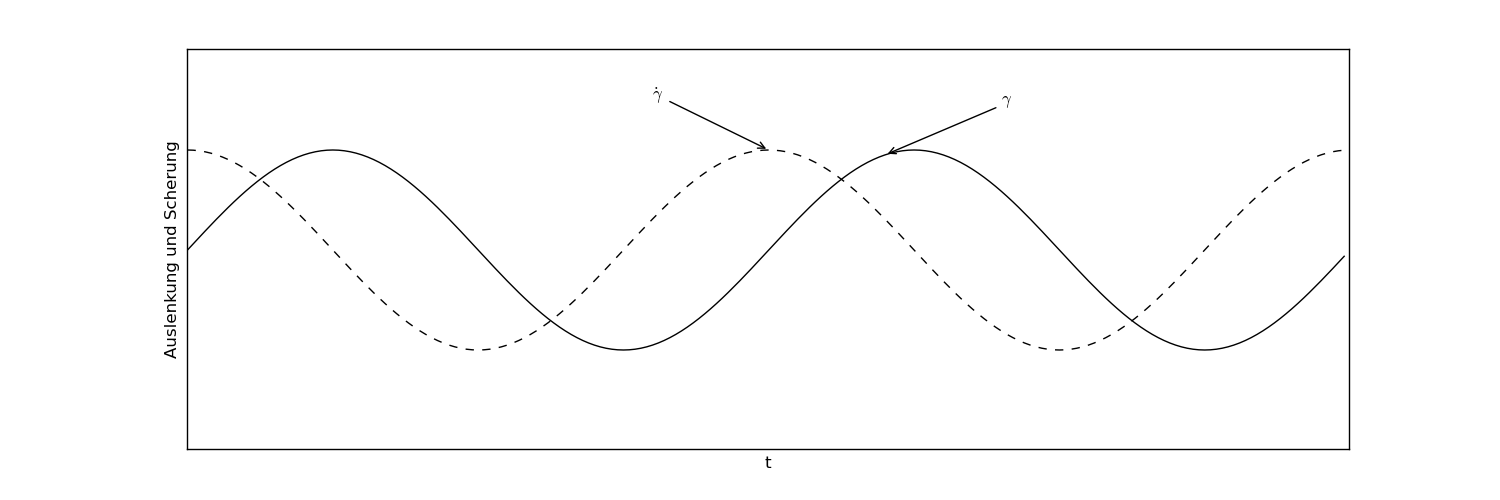
\includegraphics[width=\textwidth]{figures/SchwingungsmodiA.png}
    \label{fig:schwingungsmodi:subA}
    }\\
    \subfloat[Widerstand des Materials]{
    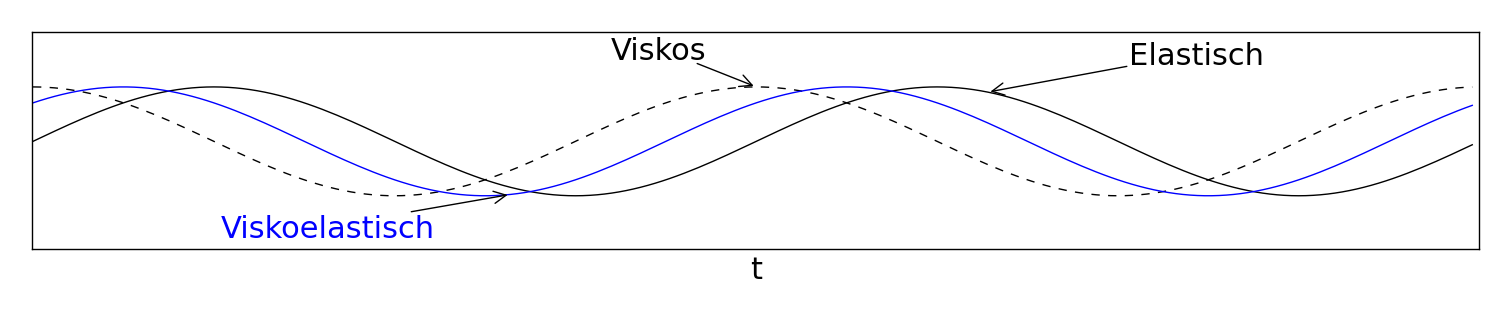
\includegraphics[width=\textwidth]{figures/SchwingungsmodiB.png}
    \label{fig:schwingungsmodi:subB}
    }
    \caption{Oszillationsversuch mit dem Platte-Platte Rheometer.\\
    In \subref{fig:schwingungsmodi:subA} ist die sinusförmige Auslenkung $\gamma$ als durchgezogene Linie, die resultierende Schergeschwindigkeit $\gammap$ als gestrichelte Linie gezeichnet.\\
    In \subref{fig:schwingungsmodi:subB} ist die Reaktion des Materials auf die Auslenkung dargestellt. Ein elastisches Material hat einen Widerstand in Phase mit der Auslenkung, eine viskose Flüssigkeit ist um 90$^\circ$ Phasenverschoben. Ein viskoelastisches Material liegt zwischen diesen beiden Kurven.
    }
    \label{fig:schwingungsmodi}
\end{figure}
%
\subsubsection{Kapillarrheometer}
Das Kapillarrheometer kann wie das Platte-Platte Rheometer zur Bestimmung der scherratenabhängigen Viskosität verwendet werden. Das Fluid wird dabei aber nicht gedreht, sondern durch eine zylinderförmige Kapillare gepresst. Als Messgrösse dient dabei der Druckunterschied.\\
Um dabei den durch das Mitmessen des Einlaufdruckverlustes (Bagley-Druck) gemachten systematischen Fehler zu korrigieren, wird meistens parallel zum eigentlichen Kapillarrheomter auch noch der Druckverlust in einer Nullblende gemessen, wie in Abbildung~(x) dargestellt. \todo{Bild Kapillarrheometer}

Die Beziehung der Messgrösse $\Delta p_{\mbox{\tiny Mess}}$ zu der Schubspannung $\tau$ ist dabei wie folgt:
\begin{equation}
    \label{eq:KapRheoTau}
    \tau\left( R \right) = \frac{R \Delta p}{2L}
\end{equation}
wobei $\Delta p = \Delta p_{\mbox{\tiny Mess}} -\Delta p_{\mbox{\tiny Bagley}}$ der korrigierte Druckunterschied ist und $L$ und $R$ die Länge respektive der Radius der Kapillare sind.

Für die Berechnung der in der Kapillare auftretenden Scherrate kann die Beziehung
\begin{equation}
    \label{eq:KapRheoScherrate}
    \gammap = \frac{4 \dot{V}}{\pi R^3}\left( \frac{3+n}{4} \right) \mbox{ mit } n=\frac{d \ln \dot{V}}{d\ln\tau}
\end{equation}
verwendet werden.

Mit Hilfe von \eqref{eq:KapRheoTau} und \eqref{eq:KapRheoScherrate} lässt sich die Fliesskurve 
\begin{equation}
    \eta(\gammap) = \frac{\tau}{\gammap}
\end{equation}
mit dem gemessenen Druckunterschied bei einem vorgegebenen Volumenstrom bestimmen.
%
%
\subsection{Korrektursimulation}
\label{Kapitel:Korrektursimulation}
Die in Kapitel \ref{Kapitel:Parameter:PlattePlatteRheo} beschriebenen Rheometer messen das für eine vorgegebene Geschwindigkeit benötigte Drehmoment. Daraus kann die Viskosität des Fluides berechnet werden.\\
Um zu verhindern, dass der Mörtel während der Messung in radialer Richtung aus dem Gerät fliesst, wurde um den Scherspalt ein Ring montiert. Dadurch wird zwar ein Herausfliessen verhindert, gleichzeitig wird aber die Messung verfälscht. Der Ring ist eine zusätzliche Wand an der das Fluid entlangströmen muss, was in ein erhöhtes Drehmoment und damit eine höhere gemessene Viskosität zur Folge hat.

Um trotzdem eine zuverlässige Bestimmung der Modell-Parameter zu ermöglichen, ist es notwendig diesen Ring im Fit zu berücksichtigen. Dazu wird nicht die gemessene Viskosität verwendet, sondern versucht die Modell-Parameter so anzupassen, dass eine Simulation des Platte-Platte Rheometers eine möglichst genaue Approximation des Drehmoments ergibt.

Beim Platte-Platte Rheometer handelt es sich um eine rotationssymmetrische Geometrie. Um Rechenzeit zu sparen wurde deshalb nur ein schmaler Ausschnitt der Geometrie simuliert, wie in Abbildung~(\ref{fig:plattePlatteRheo}) \todo{Abmessungen ins Bild einfuegen} zu sehen ist.\\
\begin{figure}
\centering
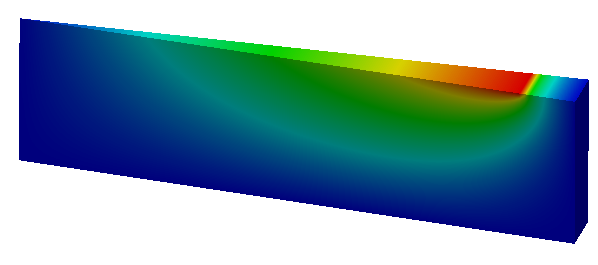
\includegraphics[width=.6\textwidth]{figures/plattenRheometerSchnitz.png}
\caption{Simulierter Teil des Platte-Platte Rheometers.\\
Eingefärbt ist das Bild nach der resultierenden Geschwindigkeitsverteilung im Rheometer.}
\label{fig:plattePlatteRheo}
\end{figure}
%
\subsection{Parameterfit}
Die in Kapitel \ref{Kapitel:Korrektursimulation} beschriebene Wahl der Parameter ist ein nichtlineares Ausgleichsproblem. Dabei soll die Gleichung \eqref{eq:modHB} möglichst gut an Mess- und Simulationsdaten gefittet werden, indem die Parameter $\tau_0$, $K$ und $n$ variiert werden.

Für die Lösung dieses Ausgleichproblemes wurde die Programmiersprache Python verwendet. Die Tatsache dass sie, ebenso wie \openfoam{}, frei verfügbar ist und dass es unzählige schon implementierte numerische Algorithmen gibt machen Python zur idealen Wahl dafür.

Die Optimierung wurde als Python Modul \codeemph{MaT\_Optimizer} implementiert. Dabei wurde auf die Bibliotheken \codeemph{Numpy} und \codeemph{Scipy} \cite{scipy} zurückgegriffen um verschiedene Standardfunktionen zur Verfügung zu haben.\\
Das Ausgleichsproblem wird dabei mittels der Funktion \codeemph{leastsq} aus dem Modul \codeemph{optimize} von \codeemph{Scipy} gelöst.
Diese Funktion ist eine Implementierung des Levenberg-Marquardt Algorithmus, der das Problem auf eine iterative Weise löst.\\
Dazu wird eine eine enge Kopplung von Python und \openfoam{} nötig, da die Auswertung der Funktion, an die gefittet werden soll, eine Reihe von Simulationen ist.

Diese Kopplung wurde dabei mit Hilfe von \codeemph{PyFoam} \cite{pyfoam} realisiert. \codeemph{PyFoam} ist eine Python Bibliothek die es ermöglicht, die von \openfoam{} als Ein- und Ausgabe benutzten Textdateien auf eine einfache Art und Weise zu erzeugen, zu ändern und auszulesen.

Um den Prozess der Parameter-Optimierung zu beschleunigen, wurde ausserdem die Bibliothek \codeemph{Parallel Python} \cite{parallelpython} verwendet. Da eine Funktionsauswertung eine ganze Reihe Simulationen beinhaltet, wird dazu viel Zeit benötigt. Diese Simulationen sind aber unabhängig voneinander und können deshalb sehr einfach parallelisiert werden. Mit \codeemph{Parallel Python} können beliebig viele Prozessoren für den Parameterfit verwendet werden.

Die gemessenen Daten des Kapillarrheometers werden bereits bei der Messung durch die Verwendung des Bagley-Druckes korrigiert. Hier muss also keine Korrektursimulation durchgeführt werden, die Daten können direkt für die Optimierung verwendet werden. Dies wird im Python Code berücksichtigt indem der Unterschied zwischen gemessenen und aus den Modell-Parametern berechneten Druckunterschiede direkt an die Fehlerfunktion angehängt wird.

Ein Beispiel für den Aufruf der Hauptfunktion \codeemph{runLeastSq}:
\begin{lstlisting}[language=Python]
plsq = runLeastSq(
      initialParam,            % Anfangssch@ä@tzer
      plateRheoTorque,         % Messdaten
      plateRheoOmega,          % Messdaten
      referenceCaseName,       % @\openfoam{}@ Case
      numberOfCpus,            % Anzahl Prozessoren
      kapRheoPressure,         % optionale Messdaten
      kapRheoShearRate         % optionale Messdaten
      ):  
\end{lstlisting}
%
Die genaue Dokumentation des Moduls kann in Anhang (x) \todo{Anhang schreiben} gefunden werden.
%
%\begin{lstlisting}[language=Python]
%plsq,res = leastsq(errFunc, initialParam, args=argList, maxfev=100)
%\end{lstlisting}
\subsection{Ergebnisse}
Die Anpassung der Parameter an gegebene Messdaten geschieht dank der Verwendung des \codeemph{MaT\_Optimizer} Moduls komplett automatisch. 
Die benötigte Zeit hängt stark von der Anzahl verwendeter Prozessoren und dem Anfangsschätzer ab.
%
\subsubsection{Verifikation}
Zur Verifikation des Verfahrens wurde einerseits die Qualität des Parameterfits anhand der vorgegebenen Messdaten beurteilt und andererseits die resultierenden Parameter für schon vermessene Mörtel mit alten Resultaten verglichen.

Der Vergleich mit alten Daten zeigt eine gute Übereinstimmung, die schon berechneten Parameter konnten mit einer Genauigkeit von unter x\% \todo{Uebereinstimmung angeben} nachgebildet werden.

Die Qualität des Fits kann anhand des von der Funktion \codeemph{leastsq} angegebenen Residuums abgeschätzt werden. Dabei zeigt sich, dass das verwendete Herschel-Bulkley Modell nicht für alle von Hilti eingesetzten Mörtel gleich gut geeignet ist. Während für die \hit{} Reihe durchwegs kleine Residuuen erreicht wurden, konnte der Algorithmus für Mörtel des \re{} Typs keine gute Übereinstimmung gefunden werden.\\
Dies liegt daran, dass das Herschel-Bulkley Modell die Eigenschaften des Mörtels nur entweder im Bereich kleiner Scherraten bis $800 s^{-1}$ oder aber im Bereich darüber nachbilden kann. Passende Parameter für alle Scherraten gibt es nicht.
%
\subsubsection{Netze}
Da die Rechenzeit einer einzelnen Simulation durch die grosse Anzahl an Simulationen sehr stark ins Gewicht fällt, wurde versucht ein so grobes Netz wie möglich zu verwenden. Natürlich wird dadurch der Diskretisierungsfehler immer grösser, weshalb ein Mittelmass zwischen benötigter Simulationszeit und gemachtem Fehler gefunden werden muss.

Dazu wurde das resultierende Drehmoment bei der Verwendung verschiedener Netze verglichen. Simuliert wurde das Platte-Platte Rheometer mit Ring, mit einer no-slip Randbedingung an der unteren Wand und am Ring, einer konstanten Drehgeschwindigkeit von 10 rad/s und einem offenen Spalt zwischen oberer Platte und dem Ring.

Das verwendete Netz, dargestellt in Abbildung~\ref{fig:PlatteRheoGitter:subA} ist ein hexaedrisches Gitter mit einer Zelle in tangentialer Richtung und einer Diskretisierungslänge von $2^{-h} \cdot 0.2\mbox{mm}$, wobei $h\in\left\{ 0,1,2,3,4 \right\}$.
%
\begin{figure}
    \centering
    \subfloat[Quadratisches Netz]{
    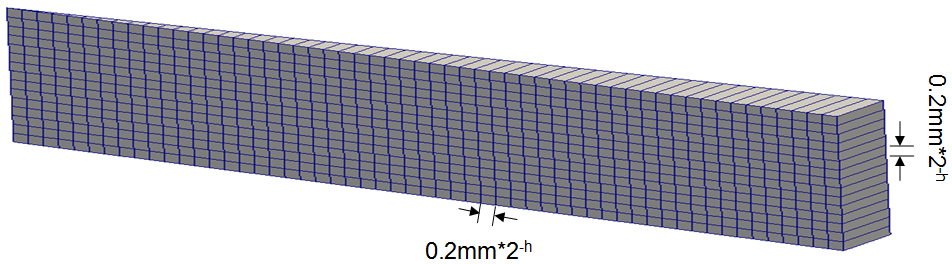
\includegraphics[width=\textwidth]{figures/PlatteRheoGitterAnnot.png}
    \label{fig:PlatteRheoGitter:subA}
    }\\
    \subfloat[O-Netz]{
    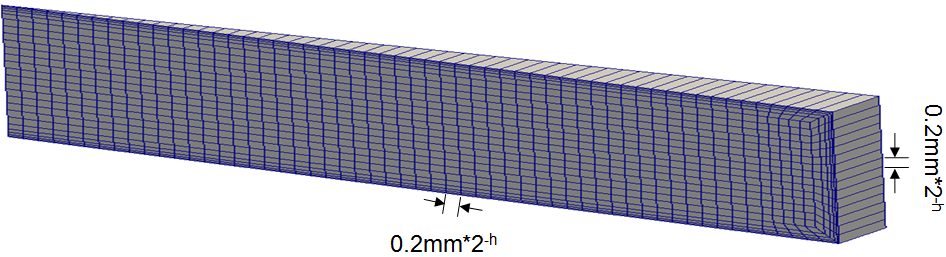
\includegraphics[width=\textwidth]{figures/PlatteRheoOGitterAnnot.png}
    \label{fig:PlatteRheoGitter:subB}
    }
    \caption{Die verwendeten Gitter für die Simulation des Platte-Platte Rheometers. \subref{fig:PlatteRheoGitter:subA} ist das quadratische Netz, \subref{fig:PlatteRheoGitter:subB} das O-Netz.
    Der Parameter $h$ wurde zwischen 0 und 4 variiert.}
    \label{fig:PlatteRheoGitter}
\end{figure}
%

Ebenfalls untersucht wurde das Verhalten des Drehmoments bei einer Verfeinerung der Netz-Randschicht. Dazu wurde ein O-Netz mit verfeinerter Randschicht verwendet, wie in Abbildung~\ref{fig:PlatteRheoGitter:subB} zu sehen ist.

Die resultierenden Werte für das Drehmoment sind in Tabelle \ref{fig:ResultingTorque} aufgeführt. Aufgrund der hohen Rechenzeit für feinere Auflösungen wurde entschieden, die Simulationen mit dem Netz $h=1$ durchzuführen.
%
\begin{table}
    \centering
    \begin{tabular}{r r r r r r}
        \textbf{h} \vline & 0 & 1 & 2 & 3 & 4\\
        \hline
        \textbf{Quadr. Netz} \vline & 1.4178e-3 & 1.4353e-3 & 1.4443e-3 & 1.4479e-3 & ?.????e-3\\
        \textbf{O-Netz} \vline & 1.4381e-3 & 1.4531e-3 & 1.4514e-3 & 1.4377e-3 & ?.????e-3
    \end{tabular}
    \caption{Resultierendes Drehmoment für verschiedene Netzauflösungen.\\
    In der ersten Zeile ist der die Auflösung bestimmende Parameter h aufgeführt, in der zweiten und dritten Zeile das resultierende Drehmoment für das quadratische und das O-Netz.}
    \label{fig:ResultingTorque}
\end{table}
\todo{endgueltige Werte}
%
\subsubsection{Resultierende Parameter}
Die in dieser Arbeit untersuchten Mörtel tragen die Bezeichnung \hit{} und \re{}, wobei bei beiden jeweils eine A und eine B Komponente existiert (Vergleiche Kapitel \ref{Kapitel:Auspressgeraet}).\\
In Tabelle \ref{fig:resultParameter} ist eine Übersicht über die angepassten Materialparameter dargestellt, in Abbildung~\ref{fig:shearVisco} sind die Messwerte und der Fit in einem doppelt logarithmischen Plot der Viskosität abhängig von der Scherrate dargestellt.

Dabei schön zu sehen ist der Einfluss des Rings, der dazu führt dass die Viskositätskurve beim Platte-Platte Rheometer deutlich unter den Messpunkten durchläuft.
Hier wurde die Viskositätsmessung durch den Ring verfälscht, was bei der Simulation wieder korrigiert wurde.
\begin{table}
    \centering
    \begin{tabular}{l c l l l}
        \textbf{Mörtel} & \textbf{Komponente} & 
        \multicolumn{1}{c}{$\tau_0$} &
        \multicolumn{1}{c}{$K$} &
        \multicolumn{1}{c}{$n$} \\
        \hline
        \hline
        \multirow{2}{*}{\hit{}} & A & 199.98& 60.90& 0.62\\ 
        & B & 238.75& 34.45& 0.52\\ 
        \hline
        \multirow{2}{*}{\re{}}  & A & 108.85& 35.22& 0.71\\ 
        & B & 134.39& 37.83& 0.62
    \end{tabular}
    \caption{Übersicht über die verwendeten Modellparameter für das Herschel-Bulkley Modell}
    \label{fig:resultParameter}
\end{table}
%
\begin{figure}
    \centering
    \subfloat[\hit{} A]{
        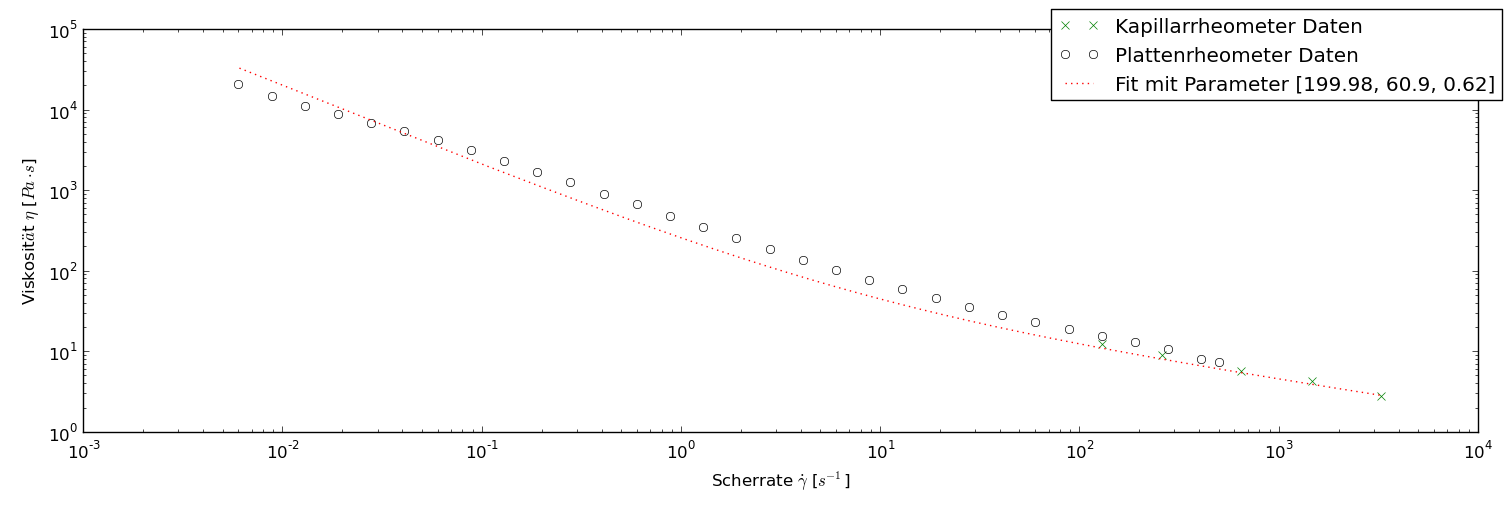
\includegraphics[width=0.47\textwidth]{figures/shearViscoMaxA.png}
        \label{fig:shearViscoHY:subA}
    }
    \subfloat[\hit{} B]{
        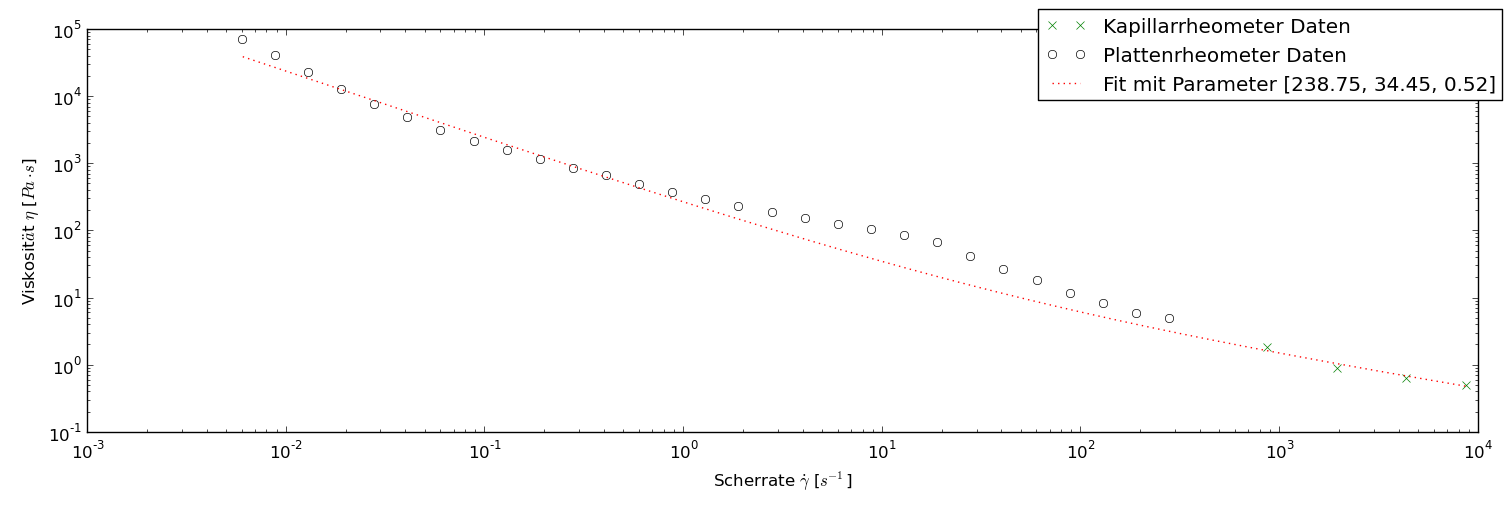
\includegraphics[width=0.47\textwidth]{figures/shearViscoMaxB.png}
        \label{fig:shearViscoHY:subB}
    } \\
    \subfloat[\re{} A]{
        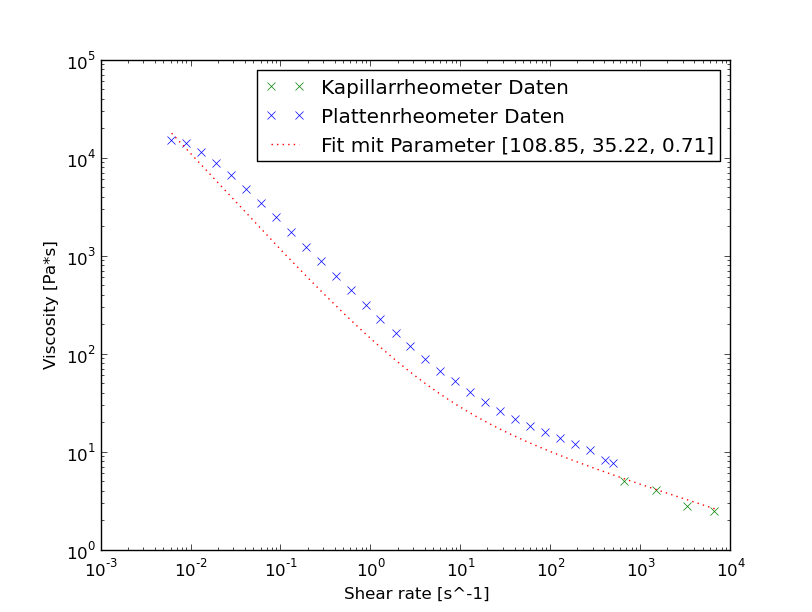
\includegraphics[width=0.47\textwidth]{figures/shearViscoReA.png}
        \label{fig:shearViscoRE:subA}
    }
    \subfloat[\re{} B]{
        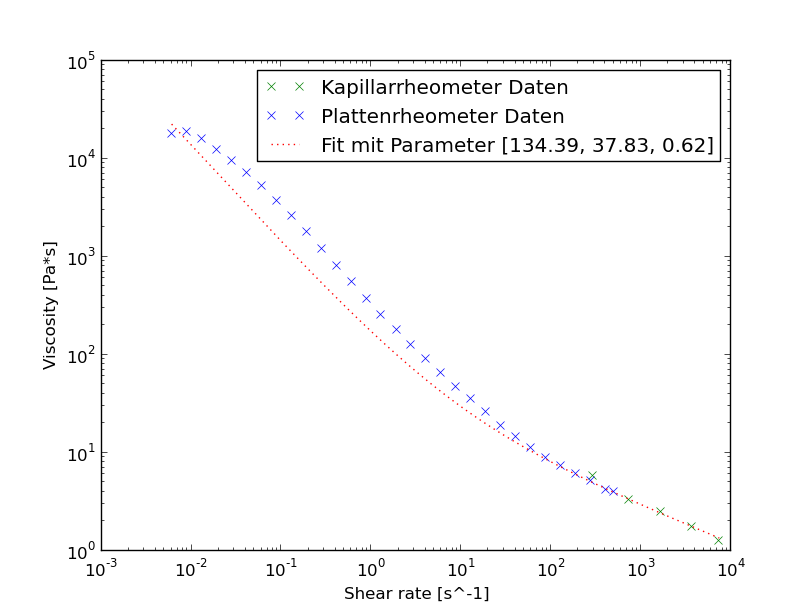
\includegraphics[width=0.47\textwidth]{figures/shearViscoReB.png}
        \label{fig:shearViscoRE:subB}
    }
    \caption{Viskosität abhängig von der Scherrate der Mörtel.\\Die Kreuze sind Messpunkte aus den beiden Rheometern, die rote Kurve der daran angepasste Fit.}
    \label{fig:shearVisco}
\end{figure}
%
\subsubsection{Relaxationszeit}
Bei den Simulationen mit dem viskoelastischen White-Metzner Materialmodell \eqref{eq:whiteMetznerModell} wird zusätzlich zu der scherratenabhängigen Viskosität auch ein Modell für die Relaxationszeit benötigt.\\
Das dazu verwendete Carreau-Yassuda Modell \eqref{eq:carreauYasuda} benötigt die fünf Parameter $\eta_{\inf}$, $\eta_0$, $L$, $\alpha$ und $n_{\lambda}$. Da die Messung der Relaxationszeit keine Korrektursimulation benötigt, kann das Modell direkt an die Messdaten gefittet werden.
Dazu wurde ebenfalls die Python-Funktion \codeemph{leastsq} verwendet. Die resultierenden Werte sind in Tabelle \ref{fig:relaxParameter} dargestellt, in Abbildung~\ref{fig:shearLambda} sind die Messpunkte und der entsprechende Fit in einem Relaxationszeit - Scherraten Diagramm gezeigt.
\begin{table}
    \centering
    \begin{tabular}{l c l l l l l}
        \textbf{Mörtel} & 
        \textbf{Komponente} & 
        \multicolumn{1}{c}{$\eta_{\inf}$} & 
        \multicolumn{1}{c}{$\eta_0$} &
        \multicolumn{1}{c}{$L$} & 
        \multicolumn{1}{c}{$n_{\lambda}$} & 
        \multicolumn{1}{c}{$\alpha$} \\
        \hline
        \hline
        \multirow{2}{*}{\hit{}} & A & 0.01   & 3.81  & 15.97 & 0.05 & 3       \\ 
                                & B & 0.002  & 0.18  & 40.12 & 0.65 & 1.8     \\ 
        \hline
        \multirow{2}{*}{\re{}}  & A & 0.0012 & 9.43 & 26.37  & 0.13 & 1.64    \\ 
                                & B & 0.01   & 7.8  & 70.12  & 0.04 & 2.3         
    \end{tabular}
    \caption{Übersicht über die verwendeten Modellparameter für das Carreau-Yasuda Modell}
    \label{fig:relaxParameter}
\end{table}
%
\begin{figure}
    \centering
    \subfloat[\hit{} A]{
        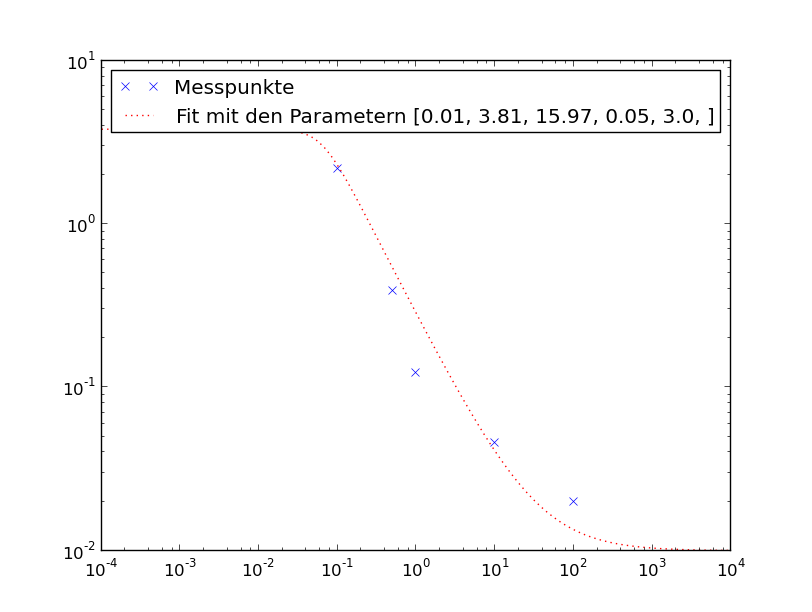
\includegraphics[width=0.47\textwidth]{figures/shearLambdaMaxA.png}
        \label{fig:shearLambdaHY:subA}
    }
    \subfloat[\hit{} B]{
        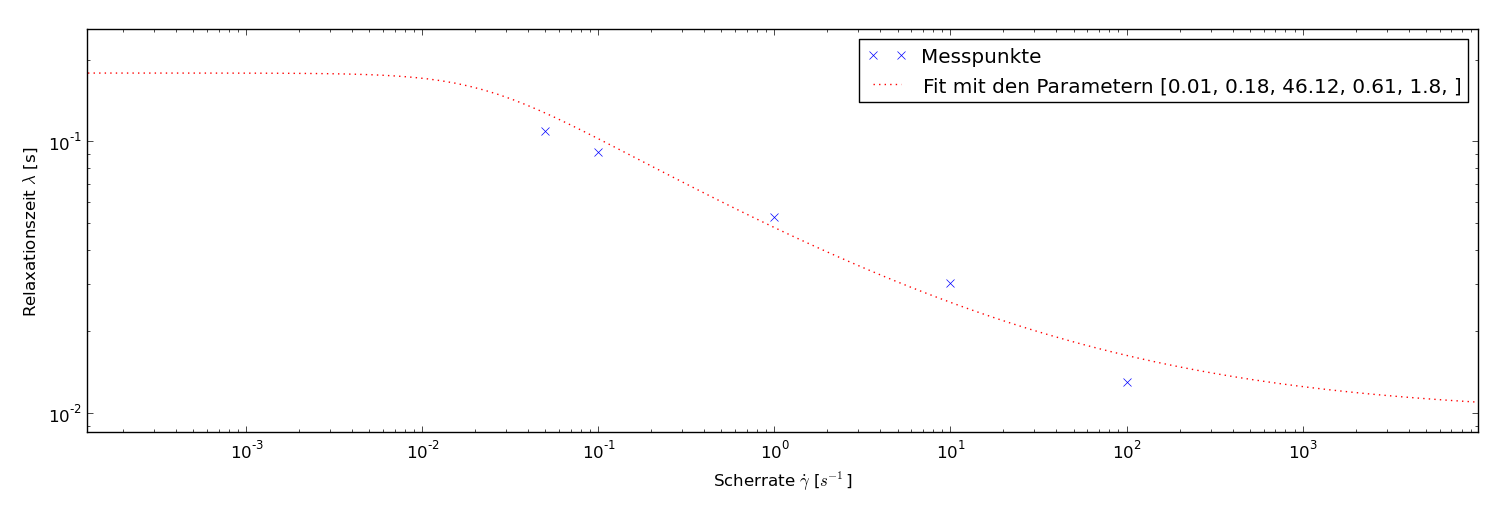
\includegraphics[width=0.47\textwidth]{figures/shearLambdaMaxB.png}
        \label{fig:shearLambdaHY:subB}
    } \\
    \subfloat[\re{} A]{
        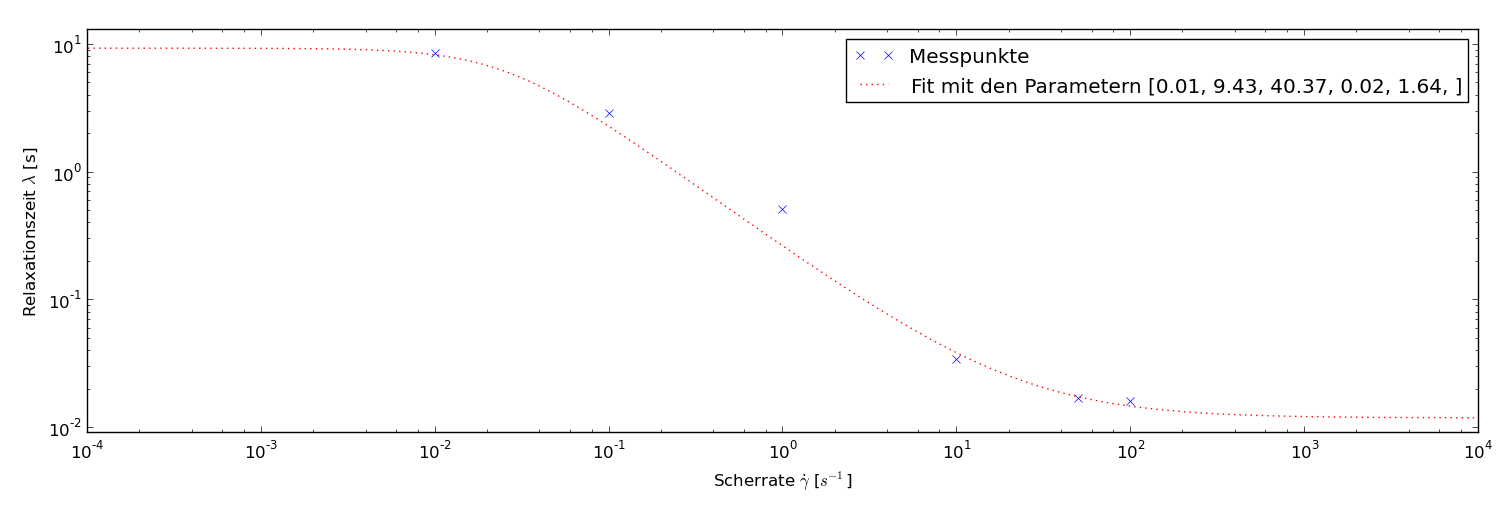
\includegraphics[width=0.47\textwidth]{figures/shearLambdaReA.png}
        \label{fig:shearLambdaRE:subA}
    }
    \subfloat[\re{} B]{
        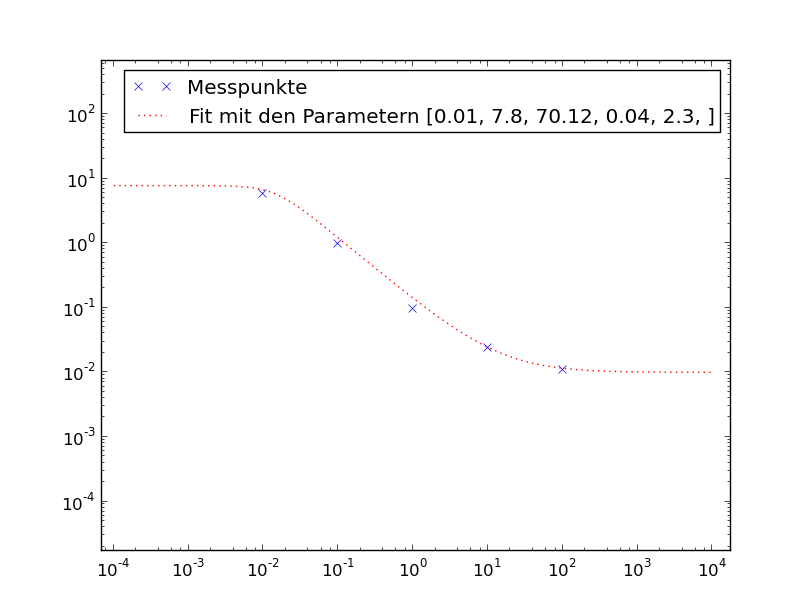
\includegraphics[width=0.47\textwidth]{figures/shearLambdaReB.png}
        \label{fig:shearLambdaRE:subB}
    }
    \caption{Relaxationszeit abhängig von der Scherrate der Mörtel.\\Die Kreuze sind Messpunkte aus der Rheometermessung, die rote Kurve der daran angepasste Fit.}
    \label{fig:shearLambda}
\end{figure}
%
\subsubsection{Simulation Kapillarrheometer}
Das Kapillarrheometer musste für die Anpassung der Parameter nicht simuliert werden. Um eine weitere Kontrollmöglichkeit über die Verlässlichkeit der Parameter zu haben wurden deshalb Simulationen des Kapillarrheometers mit Messwerten verglichen.

Zur Vermessung des Mörtels wurden zwei Kapillarrheometer mit verschiedenen Kapillaren verwendet. Die eine hat eine Länge von $L=32\mbox{mm}$ und einen Durchmesser von $R=1\mbox{mm}$, während die andere mit $L=16\mbox{mm}$ und $R=0.5\mbox{mm}$ nur halb so gross ist.\\
Dabei wurden sowohl Simulationen mit dem rein scherratenabhängigen Modell als auch mit dem viskoelastischen Materialmodell durchgeführt.

Die Simulation wurde Aufgrund der rotationssymmetrischen Geometrie ebenfalls nur für einen fünf Grad Schnitz \todo{Ausdruck Schnitz} des Rheometers durchgeführt, wie in Abbildung~\ref{fig:kapRheo} \todo{Bild} zu sehen ist.\\
Das verwendete Netz wurde so skaliert, dass die Auflösung nahe an der Einlassdüse zur Kapillare sehr fein Aufgelöst ist, während in Regionen die weit von der Düse entfernt sind eine eher grobe Auflösung verwendet wurde.

Zur Untersuchung des Einfluss der harten Kannte an der Einlassdüse wurde zusätzlich noch ein Netz mit einer abgerundeten Kante simuliert. (Abbildung~\ref{fig:roundMesh}) \todo{Einfluss Rundung} \todo{Bild}

Die Resultate sind in Tabelle \ref{fig:kapRheoResults} aufgefueh;rt.

\begin{todocontent}
    \1 Einfluss visco
\end{todocontent}
%
